\begin{center}
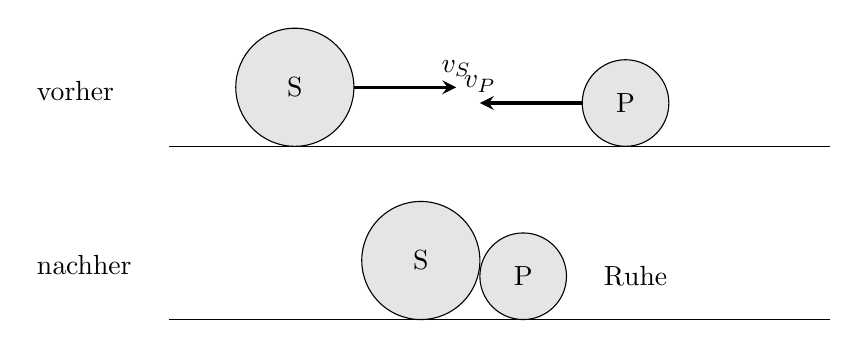
\begin{tikzpicture}[>=stealth]
 \node[anchor=west] at (0,0.7) {vorher};
 \draw (1.8,0) -- (10.2,0);
 \draw[fill=gray!20] (3.4,0.75) circle (0.75);
 \node at (3.4,0.75) {S};
 \draw[->, very thick] (4.15,0.75) -- (5.45,0.75) node[above] {$v_\text{S}$};
 \draw[fill=gray!20] (7.6,0.55) circle (0.55);
 \node at (7.6,0.55) {P};
 \draw[->, very thick] (7.05,0.55) -- (5.75,0.55) node[above] {$v_\text{P}$};
 \node[anchor=west] at (0,-1.5) {nachher};
 \draw (1.8,-2.2) -- (10.2,-2.2);
 \draw[fill=gray!20] (5,-1.45) circle (0.75);
 \node at (5,-1.45) {S};
 \draw[fill=gray!20] (6.3,-1.65) circle (0.55);
 \node at (6.3,-1.65) {P};
 \node[anchor=west] at (7.2,-1.65) {Ruhe};
\end{tikzpicture}
\end{center}

Nach dem Zusammenstoss ist der Gesamtimpuls null, also war er es auch vorher: Die beiden Impulse waren gleich gross und entgegengesetzt gerichtet,
\begin{align}
 m_\text{S}\,v_\text{S} - m_\text{P}\,v_\text{P} &= 0
\end{align}
Daraus folgt
\begin{align}
 v_\text{P} &= \vPhF = \frac{\mSu\cdot\vSu}{\mPh} = \vPh \approx \result{\vPhP{0}{2}}
\end{align}
